\documentclass{beamer}
\usepackage[utf8]{inputenc}
\usepackage[T1]{fontenc}
\usepackage{lipsum, lmodern}
\usepackage{tikz}
\usepackage{hyperref}
\usepackage{graphicx}
\usepackage{animate}
\usepackage{algorithm,algorithmic}
\usepackage{optidef} %formules d'optimisation
\include{pythonlisting}

\usetikzlibrary{arrows}

\usetheme{/Milano} % or Median, or Metro, or PraterStreet, or Milano

\newtheorem{remark}[theorem]{Remark}

\author{Prateeba\\ Ruggoo}
\supervisor{Jean\\ Cardinal}
\title{Reconfiguration problems}
\subtitle{Complexity analysis}
\institute{Université Libre de Bruxelles}
\department{Department of Computer Science - ULB}
\date{\today}

\logo{
\includegraphics[scale=0.7]{img/ulbquadri_mini}}
\titlepagelogoA{
\includegraphics[scale=1.5]{img/ulbquadri_mini}}
\backgroundlogo{
\includegraphics[scale=1.4]{img/ulb}}

\begin{document}
\frame{\maketitle}
\begin{frame}{Table of contents}
	\tableofcontents
\end{frame}

\section{Introduction}

\begin{frame}{Introduction}
  \begin{block}{Introductory problem : POWER SUPPLY Problem}
  Let $C$ be a set of customers, $P$ be a set of power stations and $G = (V,E)$ be a bipartite graph where $V = \{C \cup P$\} with weights on the vertices.  \hfill \break
  \pause
  Can $G$ be partitioned into subtrees, such that each subtree contains exactly one power supply $P$ and that the demands of $P^{'}s$ customers is $\leq$ to its capacity?
  \end{block}
\end{frame}

\begin{frame}{Introduction}
\begin{columns}
    \begin{column}{0.5\textwidth}
        \begin{figure}
        \centering
        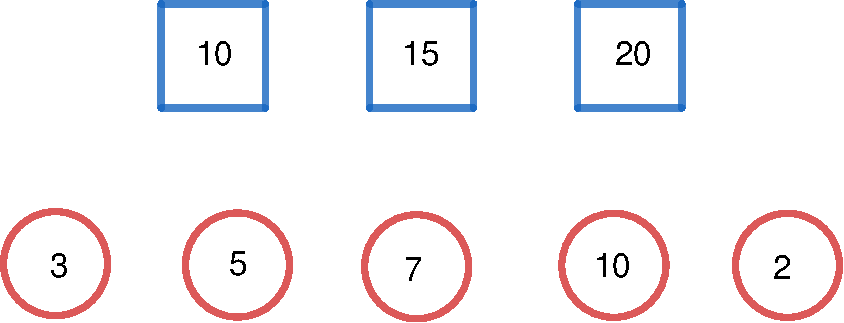
\includegraphics[width=0.9\textwidth]{img/ps1.pdf}
        \caption{Input graph $G$ where the blue vertices are the power stations and red vertices are the customers.}
        \label{fig:ps}
        \end{figure}
    \end{column}
    \pause
    \begin{column}{0.5\textwidth}
        \begin{figure}
        \centering
        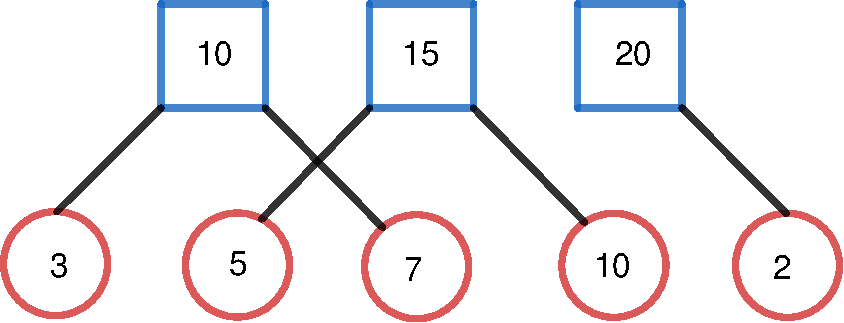
\includegraphics[width=0.9\textwidth]{img/ps2.pdf}
        \caption{A feasible solution to the POWER SUPPLY problem.\hfill \break}
        \label{fig:circle}
        \end{figure}
    \end{column}
\end{columns}

\begin{block}{Theorem}
The POWER SUPPLY problem is $\mathcal{NP}-complete$.
\end{block}
\end{frame}

\subsection{Power Supply Reconfiguration Problem}
\begin{frame}{POWER SUPPLY RECONFIGURATION Problem}
Suppose now that we are given two feasible solutions $s_0$ and $s_t$ of the POWER SUPPLY problem and are asked: Can one solution be transformed into the other by moving only one customer at a time and always remaining feasible?
\pause
\begin{columns}
    \begin{column}{0.5\textwidth}
        \begin{figure}
        \centering
        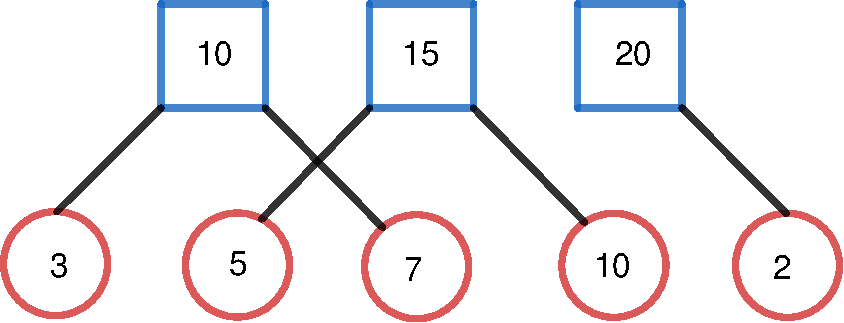
\includegraphics[width=0.9\textwidth]{img/ps2.pdf}
        \caption{Feasible solution $s_0$.}
        \label{fig:circle}
        \end{figure}
    \end{column}
    \begin{column}{0.5\textwidth}
        \begin{figure}
        \centering
        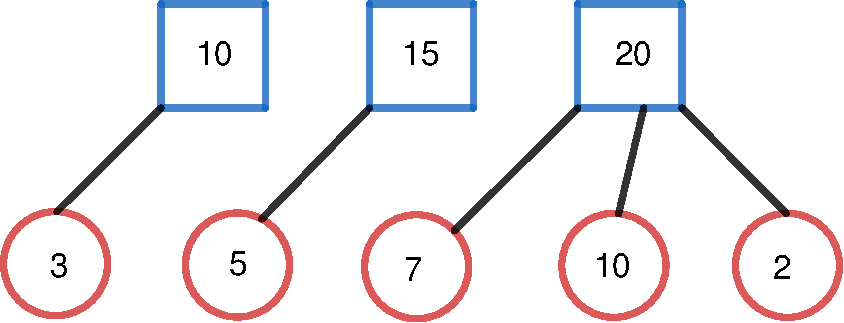
\includegraphics[width=0.9\textwidth]{img/ps4.pdf}
        \caption{Feasible solution $s_t$.}
        \label{fig:circle}
        \end{figure}
    \end{column}
\end{columns}

\end{frame}

\begin{frame}{POWER SUPPLY RECONFIGURATION Problem}
\begin{columns}
    \begin{column}{0.3\textwidth}
        \begin{figure}
        \centering
        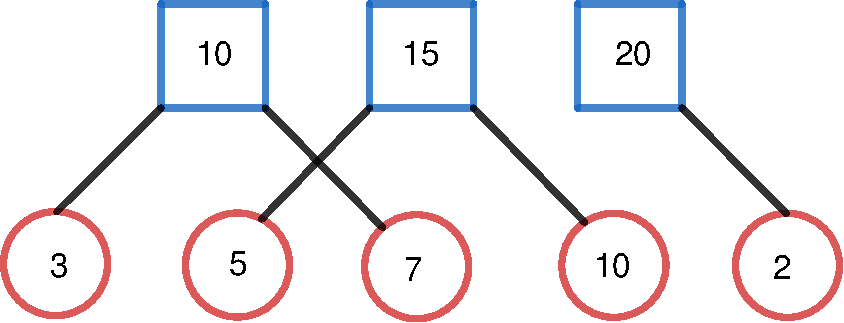
\includegraphics[width=1.1\textwidth]{img/ps2.pdf}
        \caption{Feasible solution $s_0$.\hfill \break \hfill \break \hfill \break \hfill \break}
        \label{fig:circle}
        \end{figure}
    \end{column}
    \begin{column}{0.3\textwidth}
        \begin{figure}
        \centering
        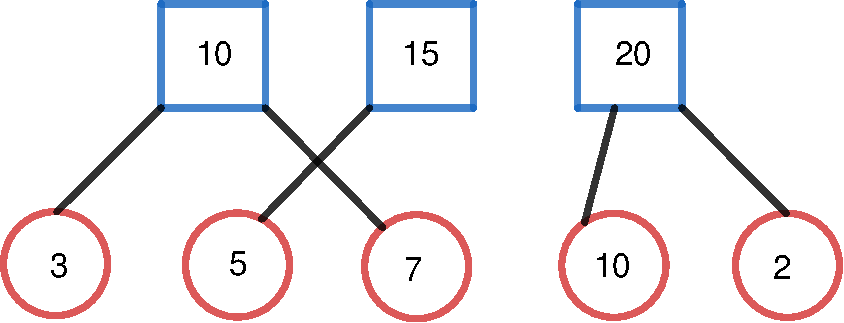
\includegraphics[width=1.1\textwidth]{img/ps3.pdf}
        \caption{Intermediate feasible solution $s_i$ where customer $10$ is moved.\hfill \break \hfill \break}
        \label{fig:circle}
        \end{figure}
    \end{column}
    \begin{column}{0.3\textwidth}
        \begin{figure}
        \centering
        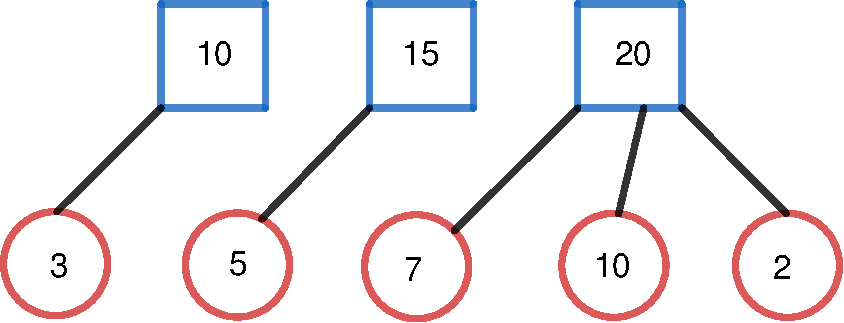
\includegraphics[width=1.1\textwidth]{img/ps4.pdf}
        \caption{Target feasible solution $s_t$ where customer $7$ is moved from previous intermediate solution.\hfill \break}
        \label{fig:circle}
        \end{figure}
    \end{column}
\end{columns}

\begin{block}{Theorem}
POWER SUPPLY RECONFIGURATION problem is $PSPACE-complete$.
\end{block}

\end{frame}

\section{Reconfiguration problems}
\begin{frame}{RECONFIGURATION problems}
  \begin{block}{Defintion}
    Given two combinatorial configurations satisfying a problem while satisfying some constraints, is it possible to transform one configuration to another by modifying only one element at a time and that the intermediate solution remains satisfiable at all times.
  \end{block}
\end{frame}


\begin{frame}{Why do RECONFIGURATION problems spark interests?}
  Reconfiguration arises in countless problems that involve movement and change.
  \begin{enumerate}
    \item Problems in computational geometry such as morphing graph drawings.
    \item Problems related to games and puzzles, such as the 15-puzzle, a topic of research since 1879.
    \item Questions of evolvability: Can genotype $y_0$ evolve into genotype $y_t$ via individual mutations each of which are of
          adequate fitness?
    \item Most importantly reconfiguration problems yield insights into the structure of the solution space and connectivity of the set of feasible solutions.
  \end{enumerate}
\end{frame}

\begin{frame}{SATISFIABILITY RECONFIGURATION Problems}
  \begin{block}{SATISFIABILITY Problem}
      \begin{block}{Definition}
      The SATISFIABILITY problem, also called SAT is to test whether a Boolean formula is satisfiable. An example of a Boolean formula is $\phi = (x_1 \vee x_2 \vee \neg x_3) \wedge (x_1 \vee \neg x_2 \vee x_3)$.
      \end{block}

      \begin{block}{Theorem}
      Cook-Levin Theorem : SAT is $\mathcal{NP}-complete.$
      \end{block}
  \end{block}

\end{frame}

\subsection{Satisfiability Reconfiguration Problems}
\begin{frame}{SATISFIABILITY RECONFIGURATION Problems}
  \begin{block}{The SAT RECONFIGURATION problem}
      \begin{block}{Definition}
      Given a boolean formula $\phi$ and two feasible solutions $s_0$ and $s_t$, is there a way to transform the feasible solution $s_0$ to $s_t$ while maintaining the two following constraints:
      \pause
      \begin{enumerate}
          \item At each step, only one variable $x_i$ of the boolean formula can be flipped.
          \item Each intermediate solution $x_k$ must be feasible.
      \end{enumerate}
      \end{block}

      \begin{block}{Theorem}
      SAT RECONFIGURATION problem is PSPACE-complete.
      \end{block}

  \end{block}
\end{frame}

\subsection{Complexity}
\begin{frame}{Complexity}
In general the reconfiguration problem of an $\mathcal{NP-}complete$ problem is $PSPACE-complete$.
And the reconfiguration problem of a polynomial-time solvable problem is $PSPACE$. However there are exceptions to this general rule :
\begin{enumerate}
    \item The $3-$coloring problem is $\mathcal{NP-}hard$ and its corresponding reconfiguration problem is solvable in polynomial time.
    \item The Shortest path problem is solvable in polynomial time whereas it's corresponding reconfiguration problem is PSPACE-complete.
\end{enumerate}
\end{frame}

\section{Goal}
\begin{frame}{Goal}
The goal of this thesis is to study the classifications established among the computational complexity of different
types of reconfiguration problems. \\
And to find more about the properties of host problems that result in the pattern (seen in the previous slide) holding or not.
\end{frame}

\section{Open questions}
\begin{frame}{Open Questions}
  \begin{enumerate}
    \item What is the connection between the complexity of reconfiguration problems and the complexity of the decision problem on the existence of configurations of a particular kind ?
    \item Is the TRAVELLING SALESMAN RECONFIGURATION problem (where two tours are adjacent if they differ in two edges) PSPACE-
    complete?
    \item What are the properties of host problems that result in the general pattern holding or not?
  \end{enumerate}

\end{frame}

%\section{Satisfiability reconfiguration problems}

\begin{frame}{Satisfiability reconfiguration problems}
  \begin{block}{Definition}
  Given a boolean formula $\phi$ with $n$ boolean variables $\{x_i,x_{i+1}, \dots, x_n\}$ with $i = \{0,\dots, n\}$ and two configurations $s_0$, $s_t$ from $\{T,F\}^{n}$ that satisfy $\phi$, is there a way to transform one configuration to the other with the following constraints:
  \begin{enumerate}
      \item At each step, only one variable $x_i$ can be flipped.
      \item Each intermediate configuration $x_k$ must be feasible i.e satisfy $\phi$.
  \end{enumerate}
  \end{block}

\end{frame}

%\section{Binary Integer programming Reconfiguration problems}
\subsection{Constrained Hypercube Path Problem}

\begin{frame}{Constrained Hypercube Path Problem}
  The constrained hypercube path can be seen as a reconfiguration analogue to the $0 − 1$
  Integer programming problem.

  \begin{block}{$0 − 1$ Integer programming problem Definition}

  \end{block}

\end{frame}



\thanksframe{Thank you for your attention \\
The slides, resources and report can be found at: \\
\url{https://github.com/Prateeba/MEMO-F403}
}


\end{document}
